\section{Diskussion der Ergebnisse}
\label{sec:diskussion}

Es zeigt sich, dass es grundlegend möglich ist nur die aufgehende Struktur zu modellieren und anhand der Isolationsspektren eine Modalanalyse durchzuführen.
Dabei werden die Parameter des Isolators erfasst um ein modifiziertes Antwortspektrum zu erzeugen.
Es wird aber auch deutlich, dass wie bereits erwähnt, der vereinfachte Ansatz für Perioden in der Nähe der Isolatorperiode auf der unsicheren Seite und der Ansatz über die Transmissibilität deutlich auf der sicheren Seite liegt.

\section{Variation des Reibungskoeffizienten $\mu$}
\label{sec:muvariation}

Interessant ist die Beobachtung, dass bei Variation des Reibungskoeffizienten (\cref{fig:muvariation}) deutlich wird, dass die optimale Isolation von $\mu$ abhängig ist und ab einem Grenzwert ein negativer Effekt eintritt.

\begin{figure}[H]
    \centering
    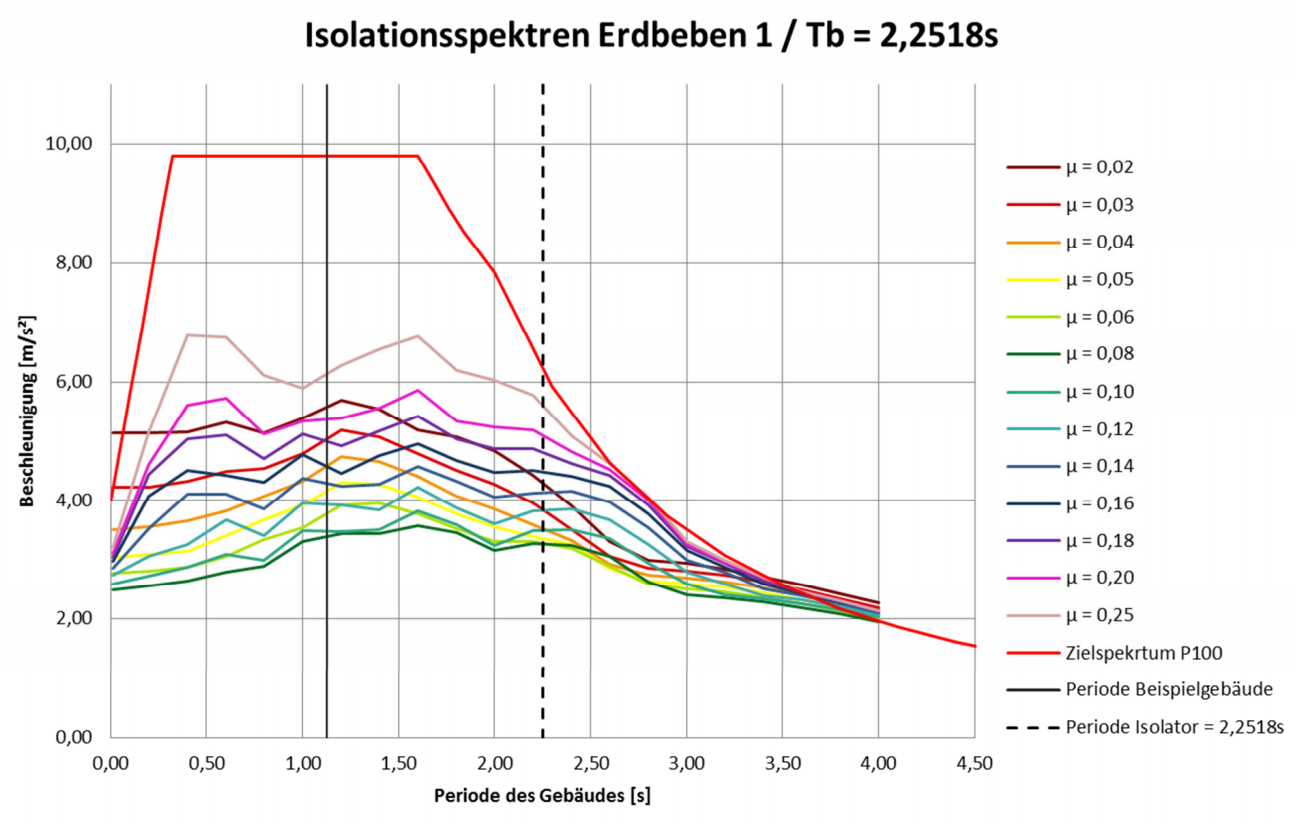
\includegraphics[width=1.0\textwidth]{variation_mu.png}
    \caption{Bild 10.10: Vergleich der Isolationsspektren des „Erdbeben 1“ bei verschiedenen Reibungskoeffizienten \cite{Isemann}}
    \label{fig:muvariation}
\end{figure}

Dieser Effekt kann mit dem vereinfachten Verfahren und dem über die Transmissibilität nicht abgebildet werden. Das liegt daran, dass bei diesen Verfahren $\mu$ einen direkten linearen Einflus auf die effektive Steifigkeit (\cref{keff}) und Dämpfung (\cref{xieff}) hat.

\begin{equation*}
k_{eff} = \frac{G}{R} + \mu \frac{G}{D}
\end{equation*}

\begin{equation*}
\xi_{eff} = \frac{2}{\pi} \frac{\mu R}{(D + \mu R)}
\end{equation*}

Er geht also bei der Linearisierung verloren und kann nur von nicht-linearen Berechnungen, oder empirischen Korrekturfaktoren abgebildet werden.

\pagebreak

\section{Ansätze für verschiende Dämpfungskorrekturbeiwerte $\eta$}

Wie in \cref{sec:Korrekturansaetze} schon erwähnt, wurde in \cite{Isemann} auch eine Korrektur über andere Ansätze für die Bestimmung des Dämpfungskorrekturbeiwertes $\eta$ untersucht.
Der Eurcode 8 sieht dabei folgende Bestimmungsgleichung vor.

\begin{equation*}
\eta = \sqrt{\frac{10}{5+\xi}}
\end{equation*}

Betrachtet man aber die Gleichung für den Vergrößerungsfaktor eines Einmassenschwingers

\begin{equation}
\frac{u_{max}}{u_{stat}} = \frac{1}{\sqrt{(1 - (\omega / \omega_1)^2)^2 + (2 \xi \omega / \omega_1)^2}}
\end{equation}

so ergibt sich im Resonanzfall für $\omega = \omega_1$, nach Umstellung die Beziehung

\begin{equation}
\eta = \frac{1}{2\xi}
\end{equation}

Für $\mu = 0.05$ und $R = 2 m$ zeigt sich aber auch hier, dass die Werte überkorrigiert werden und deutlich zu geringe Beschleunigungen liefern.

\begin{figure}[H]
    \centering
    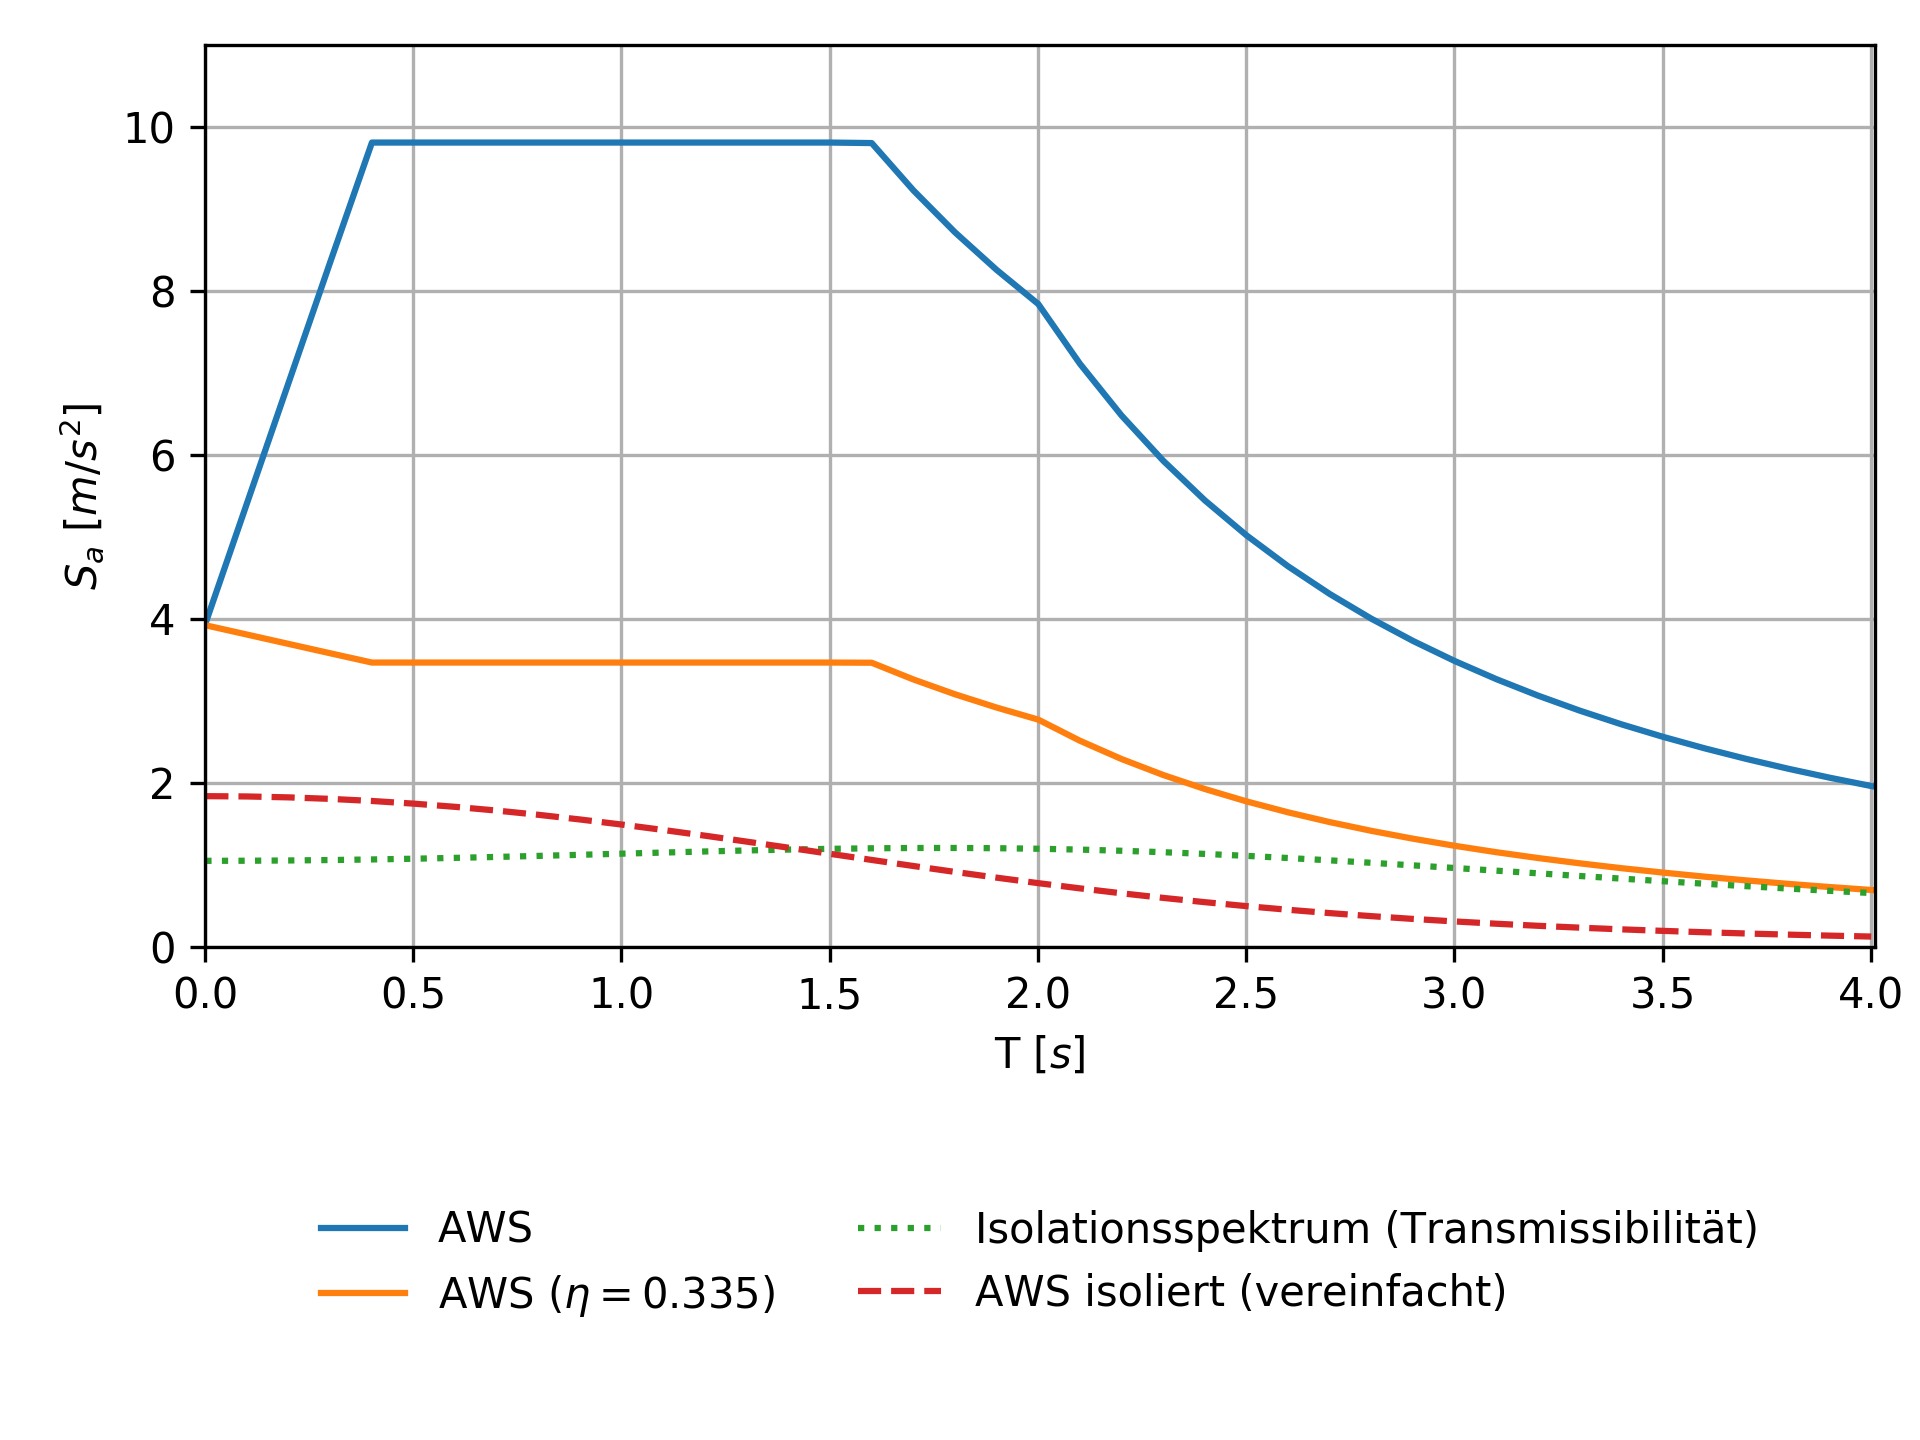
\includegraphics[width=1.0\textwidth]{Isolation_5.png}
    \caption{}
    \label{fig:Isolation5}
\end{figure}

Nun könnte eine empirische Korrektur vorgenommen werden, die die Ergebnisse aus einer Zeitschrittberechnung mit einfließen lässt. Da diese aber von den Parametern des Bauwerks abhängig sind, wurde an dieser Stelle darauf verzichtet, weil das Ziel sein sollte Isolationsspektren ohne die Erforderniss einer Zeitschrittberechnung zu erstellen.

\pagebreak